\PassOptionsToPackage{unicode=true}{hyperref} % options for packages loaded elsewhere
\PassOptionsToPackage{hyphens}{url}
%
\documentclass[]{ctexart}
\usepackage{lmodern}
\usepackage{amssymb,amsmath}
\usepackage{ifxetex,ifluatex}
\usepackage{fixltx2e} % provides \textsubscript
\ifnum 0\ifxetex 1\fi\ifluatex 1\fi=0 % if pdftex
  \usepackage[T1]{fontenc}
  \usepackage[utf8]{inputenc}
  \usepackage{textcomp} % provides euro and other symbols
\else % if luatex or xelatex
  \usepackage{unicode-math}
  \defaultfontfeatures{Ligatures=TeX,Scale=MatchLowercase}
\fi
% use upquote if available, for straight quotes in verbatim environments
\IfFileExists{upquote.sty}{\usepackage{upquote}}{}
% use microtype if available
\IfFileExists{microtype.sty}{%
\usepackage[]{microtype}
\UseMicrotypeSet[protrusion]{basicmath} % disable protrusion for tt fonts
}{}
\IfFileExists{parskip.sty}{%
\usepackage{parskip}
}{% else
\setlength{\parindent}{0pt}
\setlength{\parskip}{6pt plus 2pt minus 1pt}
}
\usepackage{hyperref}
\hypersetup{
            pdfborder={0 0 0},
            breaklinks=true}
\urlstyle{same}  % don't use monospace font for urls
\usepackage{color}
\usepackage{fancyvrb}
\newcommand{\VerbBar}{|}
\newcommand{\VERB}{\Verb[commandchars=\\\{\}]}
\DefineVerbatimEnvironment{Highlighting}{Verbatim}{commandchars=\\\{\}}
% Add ',fontsize=\small' for more characters per line
\newenvironment{Shaded}{}{}
\newcommand{\AlertTok}[1]{\textcolor[rgb]{1.00,0.00,0.00}{\textbf{#1}}}
\newcommand{\AnnotationTok}[1]{\textcolor[rgb]{0.38,0.63,0.69}{\textbf{\textit{#1}}}}
\newcommand{\AttributeTok}[1]{\textcolor[rgb]{0.49,0.56,0.16}{#1}}
\newcommand{\BaseNTok}[1]{\textcolor[rgb]{0.25,0.63,0.44}{#1}}
\newcommand{\BuiltInTok}[1]{#1}
\newcommand{\CharTok}[1]{\textcolor[rgb]{0.25,0.44,0.63}{#1}}
\newcommand{\CommentTok}[1]{\textcolor[rgb]{0.38,0.63,0.69}{\textit{#1}}}
\newcommand{\CommentVarTok}[1]{\textcolor[rgb]{0.38,0.63,0.69}{\textbf{\textit{#1}}}}
\newcommand{\ConstantTok}[1]{\textcolor[rgb]{0.53,0.00,0.00}{#1}}
\newcommand{\ControlFlowTok}[1]{\textcolor[rgb]{0.00,0.44,0.13}{\textbf{#1}}}
\newcommand{\DataTypeTok}[1]{\textcolor[rgb]{0.56,0.13,0.00}{#1}}
\newcommand{\DecValTok}[1]{\textcolor[rgb]{0.25,0.63,0.44}{#1}}
\newcommand{\DocumentationTok}[1]{\textcolor[rgb]{0.73,0.13,0.13}{\textit{#1}}}
\newcommand{\ErrorTok}[1]{\textcolor[rgb]{1.00,0.00,0.00}{\textbf{#1}}}
\newcommand{\ExtensionTok}[1]{#1}
\newcommand{\FloatTok}[1]{\textcolor[rgb]{0.25,0.63,0.44}{#1}}
\newcommand{\FunctionTok}[1]{\textcolor[rgb]{0.02,0.16,0.49}{#1}}
\newcommand{\ImportTok}[1]{#1}
\newcommand{\InformationTok}[1]{\textcolor[rgb]{0.38,0.63,0.69}{\textbf{\textit{#1}}}}
\newcommand{\KeywordTok}[1]{\textcolor[rgb]{0.00,0.44,0.13}{\textbf{#1}}}
\newcommand{\NormalTok}[1]{#1}
\newcommand{\OperatorTok}[1]{\textcolor[rgb]{0.40,0.40,0.40}{#1}}
\newcommand{\OtherTok}[1]{\textcolor[rgb]{0.00,0.44,0.13}{#1}}
\newcommand{\PreprocessorTok}[1]{\textcolor[rgb]{0.74,0.48,0.00}{#1}}
\newcommand{\RegionMarkerTok}[1]{#1}
\newcommand{\SpecialCharTok}[1]{\textcolor[rgb]{0.25,0.44,0.63}{#1}}
\newcommand{\SpecialStringTok}[1]{\textcolor[rgb]{0.73,0.40,0.53}{#1}}
\newcommand{\StringTok}[1]{\textcolor[rgb]{0.25,0.44,0.63}{#1}}
\newcommand{\VariableTok}[1]{\textcolor[rgb]{0.10,0.09,0.49}{#1}}
\newcommand{\VerbatimStringTok}[1]{\textcolor[rgb]{0.25,0.44,0.63}{#1}}
\newcommand{\WarningTok}[1]{\textcolor[rgb]{0.38,0.63,0.69}{\textbf{\textit{#1}}}}
\usepackage{graphicx,grffile}
\makeatletter
\def\maxwidth{\ifdim\Gin@nat@width>\linewidth\linewidth\else\Gin@nat@width\fi}
\def\maxheight{\ifdim\Gin@nat@height>\textheight\textheight\else\Gin@nat@height\fi}
\makeatother
% Scale images if necessary, so that they will not overflow the page
% margins by default, and it is still possible to overwrite the defaults
% using explicit options in \includegraphics[width, height, ...]{}
\setkeys{Gin}{width=\maxwidth,height=\maxheight,keepaspectratio}
\setlength{\emergencystretch}{3em}  % prevent overfull lines
\providecommand{\tightlist}{%
  \setlength{\itemsep}{0pt}\setlength{\parskip}{0pt}}
\setcounter{secnumdepth}{0}
% Redefines (sub)paragraphs to behave more like sections
\ifx\paragraph\undefined\else
\let\oldparagraph\paragraph
\renewcommand{\paragraph}[1]{\oldparagraph{#1}\mbox{}}
\fi
\ifx\subparagraph\undefined\else
\let\oldsubparagraph\subparagraph
\renewcommand{\subparagraph}[1]{\oldsubparagraph{#1}\mbox{}}
\fi

% set default figure placement to htbp
\makeatletter
\def\fps@figure{htbp}
\makeatother


\date{}

\begin{document}

\hypertarget{header-n200}{%
\subsection{6.程序测试}\label{header-n200}}

\hypertarget{header-n202}{%
\subsubsection{6.1测试环境}\label{header-n202}}

\begin{itemize}
\item
  测试在visual studio 2017搭建的工程中进行
\item
  需要词法分析程序能够处理无词法错误的程序并输出记号序列
\item
  需要语法分析程序能够处理无语法错误的记号序列,并输出对应的产生式序列
\end{itemize}

\hypertarget{header-n210}{%
\subsubsection{6.2测试功能}\label{header-n210}}

\begin{itemize}
\item
  有针对性地测试每一种成分的语义分析
\item
  编写包含各种语义错误的综合程序,进行最终测试,并检查语义分析遇到错误时的恢复情况
\end{itemize}

\hypertarget{header-n216}{%
\subsubsection{6.3测试情况}\label{header-n216}}

\hypertarget{header-n217}{%
\paragraph{(1)词法分析}\label{header-n217}}

\begin{enumerate}
\def\labelenumi{\arabic{enumi}.}
\item
  非法标识符错误测试

  \begin{enumerate}
  \def\labelenumii{\arabic{enumii}.}
  \item
    测试用例

\begin{Shaded}
\begin{Highlighting}[]
\KeywordTok{program}\NormalTok{ testLex(input, output);
}
\NormalTok{var
}
\NormalTok{	25i, j, tmp, size: }\DataTypeTok{integer}\NormalTok{;
}
\NormalTok{	list:}\KeywordTok{array}\NormalTok{[}\DecValTok{0}\NormalTok{..}\DecValTok{1000}\NormalTok{] }\KeywordTok{of} \DataTypeTok{integer}\NormalTok{;
}
\KeywordTok{begin}

    \KeywordTok{for}\NormalTok{ 25i := }\DecValTok{1} \KeywordTok{to}\NormalTok{ size}\DecValTok{-1}\NormalTok{ do
}
	\KeywordTok{for}\NormalTok{ j := }\DecValTok{1} \KeywordTok{to}\NormalTok{ i do
}
	    \KeywordTok{if}\NormalTok{ list[j] > list[j+}\DecValTok{1}\NormalTok{] then
}
	    \KeywordTok{begin}

\NormalTok{		    tmp := list[j];
}
\NormalTok{		    list[j] := list[j+}\DecValTok{1}\NormalTok{];
}
\NormalTok{		    list [j+}\DecValTok{1}\NormalTok{] := tmp;
}
	    \KeywordTok{end}\NormalTok{;
}


    \KeywordTok{for}\NormalTok{ 25i :=}\DecValTok{1} \KeywordTok{to}\NormalTok{ size do
}
	\KeywordTok{write}\NormalTok{(list[25i])
}
\KeywordTok{end}\NormalTok{.}
\end{Highlighting}
\end{Shaded}
  \item
    预期结果

    该错误类型为词法错误,对于代码中所定义的\textbf{"25i"}
    词法会识别出错误,要求输出的报错信息中准确输出错误类型,发生错误的行号,错误内容,并停止程序的继续运行。
  \item
    测试结果及分析

    \begin{figure}
    \centering
    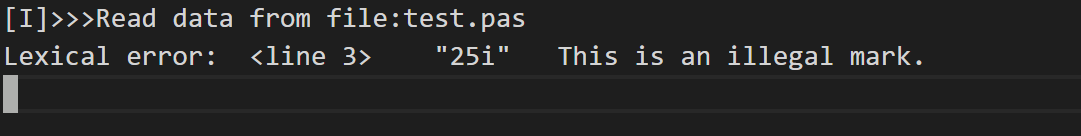
\includegraphics{C:/acm/coding/Project1/test.assets/image-20210509224301933.png}
    \caption{image-20210509224301933}
    \end{figure}
  \end{enumerate}
\item
  注释错误测试

  \begin{enumerate}
  \def\labelenumii{\arabic{enumii}.}
  \item
    测试用例

\begin{Shaded}
\begin{Highlighting}[]
\KeywordTok{program}\NormalTok{ testLex(input, output);}
\KeywordTok{var}
\NormalTok{	i, j, tmp, size: }\DataTypeTok{integer}\NormalTok{;}
\NormalTok{	list:}\KeywordTok{array}\NormalTok{[}\DecValTok{0}\NormalTok{..}\DecValTok{1000}\NormalTok{] }\KeywordTok{of} \DataTypeTok{integer}\NormalTok{;}
	\CommentTok{\{wiwqkhjk62?P@!@@8\}}\NormalTok{\}\}\}}
\KeywordTok{begin}
    \KeywordTok{for}\NormalTok{ i := }\DecValTok{1} \KeywordTok{to}\NormalTok{ size}\DecValTok{-1} \KeywordTok{do}
	\KeywordTok{for}\NormalTok{ j := }\DecValTok{1} \KeywordTok{to}\NormalTok{ i }\KeywordTok{do}
	    \KeywordTok{if}\NormalTok{ list[j] > list[j+}\DecValTok{1}\NormalTok{] }\KeywordTok{then}
	    \KeywordTok{begin}
\NormalTok{		    tmp := list[j];}
\NormalTok{		    list[j] := list[j+}\DecValTok{1}\NormalTok{];}
\NormalTok{		    list [j+}\DecValTok{1}\NormalTok{] := tmp;}
	    \KeywordTok{end}\NormalTok{;}

    \KeywordTok{for}\NormalTok{ i :=}\DecValTok{1} \KeywordTok{to}\NormalTok{ size }\KeywordTok{do}
	\KeywordTok{write}\NormalTok{(list[i])}
\KeywordTok{end}\NormalTok{.}
\end{Highlighting}
\end{Shaded}
  \item
    预期结果

    该错误类型为词法错误,对于代码中出现的的注释
    \textbf{\{wiwqkhjk62?P@!@@8\}\}\}\}}词法会识别出错误,但并不将括号内的特殊字符识别为词法错误,而是将其与左右括号一起识别为注释,真正的错误应该是最后三个无对应匹配左括号的右括号,因此要求输出的报错信息中准确输出错误类型为词法错误,发生错误的行号,错误内容为\textbf{\}\}\}},并停止程序的继续运行。
  \item
    测试结果及分析

    \begin{figure}
    \centering
    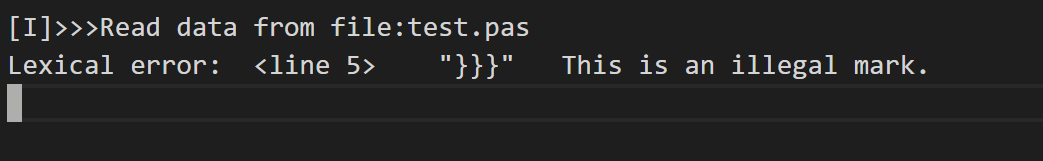
\includegraphics{C:/acm/coding/Project1/test.assets/image-20210509224413027.png}
    \caption{image-20210509224413027}
    \end{figure}
  \end{enumerate}
\item
  非法符号错误测试

  \begin{enumerate}
  \def\labelenumii{\arabic{enumii}.}
  \item
    测试用例

\begin{Shaded}
\begin{Highlighting}[]
\KeywordTok{program}\NormalTok{ testLex(input, output);}
\KeywordTok{var}
\NormalTok{	i@djdhs, j, tmp, size: }\DataTypeTok{integer}\NormalTok{;}
\NormalTok{	list:}\KeywordTok{array}\NormalTok{[}\DecValTok{0}\NormalTok{..}\DecValTok{1000}\NormalTok{] }\KeywordTok{of} \DataTypeTok{integer}\NormalTok{;	}
\KeywordTok{begin}
    \KeywordTok{for}\NormalTok{ i@djdhs := }\DecValTok{1} \KeywordTok{to}\NormalTok{ size}\DecValTok{-1} \KeywordTok{do}
	\KeywordTok{for}\NormalTok{ j := }\DecValTok{1} \KeywordTok{to}\NormalTok{ i@djdhs }\KeywordTok{do}
	    \KeywordTok{if}\NormalTok{ list[j] > list[j+}\DecValTok{1}\NormalTok{] }\KeywordTok{then}
	    \KeywordTok{begin}
\NormalTok{		    tmp := list[j];}
\NormalTok{		    list[j] := list[j+}\DecValTok{1}\NormalTok{];}
\NormalTok{		    list [j+}\DecValTok{1}\NormalTok{] := tmp;}
	    \KeywordTok{end}\NormalTok{;}

    \KeywordTok{for}\NormalTok{ i@djdhs :=}\DecValTok{1} \KeywordTok{to}\NormalTok{ size }\KeywordTok{do}
	\KeywordTok{write}\NormalTok{(list[i@djdhs])}
\KeywordTok{end}\NormalTok{.}
\end{Highlighting}
\end{Shaded}
  \item
    预期结果

    该错误类型为词法错误,对于代码中所定义的\textbf{"i@djdhs"}
    词法会识别出非法符号\textbf{@},要求输出的报错信息中准确输出错误类型,发生错误的行号,错误内容,并停止程序的继续运行。
  \item
    测试结果及分析

    对于非法符号,为了避免繁杂只给出了对\textbf{@}的测试,但实际上词法对错误符号的识别支持@、\#、¥、!、+、*等

    \begin{figure}
    \centering
    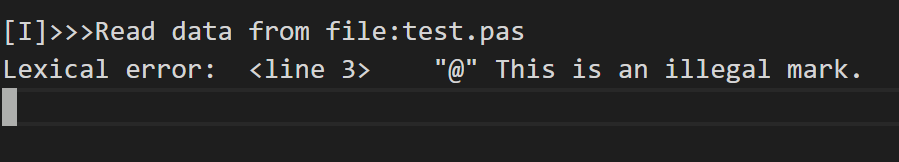
\includegraphics{C:/acm/coding/Project1/test.assets/image-20210509224503614.png}
    \caption{image-20210509224503614}
    \end{figure}
  \end{enumerate}
\item
  字符长度超标错误测试

  \begin{enumerate}
  \def\labelenumii{\arabic{enumii}.}
  \item
    测试用例

\begin{Shaded}
\begin{Highlighting}[]
\KeywordTok{program}\NormalTok{ testLex(input, output);}
\KeywordTok{var}
\NormalTok{	i, j, tmp, size: }\DataTypeTok{integer}\NormalTok{;}
\NormalTok{	list:}\KeywordTok{array}\NormalTok{[}\DecValTok{0}\NormalTok{..}\DecValTok{1000}\NormalTok{] }\KeywordTok{of} \DataTypeTok{integer}\NormalTok{;	}
\NormalTok{	dgqwyudqkjdbuywqeihlqwjdhskdbwjbkduowqhlwddwwegdehkkhwkdgwljdlwjdew: }\DataTypeTok{integer}\NormalTok{;}
\KeywordTok{begin}
    \KeywordTok{for}\NormalTok{ i := }\DecValTok{1} \KeywordTok{to}\NormalTok{ size}\DecValTok{-1} \KeywordTok{do}
	\KeywordTok{for}\NormalTok{ j := }\DecValTok{1} \KeywordTok{to}\NormalTok{ i }\KeywordTok{do}
	    \KeywordTok{if}\NormalTok{ list[j] > list[j+}\DecValTok{1}\NormalTok{] }\KeywordTok{then}
	    \KeywordTok{begin}
\NormalTok{		    tmp := list[j];}
\NormalTok{		    list[j] := list[j+}\DecValTok{1}\NormalTok{];}
\NormalTok{		    list [j+}\DecValTok{1}\NormalTok{] := tmp;}
	    \KeywordTok{end}\NormalTok{;}

    \KeywordTok{for}\NormalTok{ i :=}\DecValTok{1} \KeywordTok{to}\NormalTok{ size }\KeywordTok{do}
	\KeywordTok{write}\NormalTok{(list[i])}
\KeywordTok{end}\NormalTok{.}
\end{Highlighting}
\end{Shaded}
  \item
    预期结果

    该错误类型为词法错误,由于设定的pascal语言对于标识符和数字的长度最大长度为32位,对于代码中出现的\textbf{dgqwyudqkjdbuywqeihlqwjdhskdbwjbkduowqhlwddwwegdehkkhwkdgwljdlwjdew},长度超过了32位,故会识别出词法错误,要求输出的报错信息中准确输出错误类型,发生错误的行号,错误内容,并停止程序的继续运行。
  \item
    测试结果及分析

    \begin{figure}
    \centering
    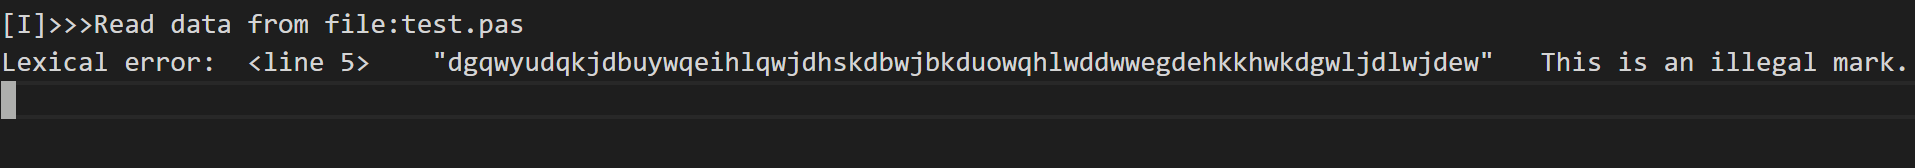
\includegraphics{C:/acm/coding/Project1/test.assets/image-20210509224606734.png}
    \caption{}
    \end{figure}
  \end{enumerate}
\item
  字符符号内为字符串错误测试

  \begin{enumerate}
  \def\labelenumii{\arabic{enumii}.}
  \item
    测试用例

    \begin{enumerate}
    \def\labelenumiii{\arabic{enumiii}.}
    \item
\begin{Shaded}
\begin{Highlighting}[]
\KeywordTok{program}\NormalTok{ testLex(input, output);}
\KeywordTok{const} 	
\NormalTok{	ch = }\StringTok{'hwqywu'}\NormalTok{;}
\KeywordTok{var}
\NormalTok{	i, j, tmp, size: }\DataTypeTok{integer}\NormalTok{;}
\NormalTok{	list:}\KeywordTok{array}\NormalTok{[}\DecValTok{0}\NormalTok{..}\DecValTok{1000}\NormalTok{] }\KeywordTok{of} \DataTypeTok{integer}\NormalTok{;}

\KeywordTok{begin}
    \KeywordTok{for}\NormalTok{ i := }\DecValTok{1} \KeywordTok{to}\NormalTok{ size}\DecValTok{-1} \KeywordTok{do}
	\KeywordTok{for}\NormalTok{ j := }\DecValTok{1} \KeywordTok{to}\NormalTok{ i }\KeywordTok{do}
	    \KeywordTok{if}\NormalTok{ list[j] > list[j+}\DecValTok{1}\NormalTok{] }\KeywordTok{then}
	    \KeywordTok{begin}
\NormalTok{		    tmp := list[j];}
\NormalTok{		    list[j] := list[j+}\DecValTok{1}\NormalTok{];}
\NormalTok{		    list [j+}\DecValTok{1}\NormalTok{] := tmp;}
	    \KeywordTok{end}\NormalTok{;}

    \KeywordTok{for}\NormalTok{ i :=}\DecValTok{1} \KeywordTok{to}\NormalTok{ size }\KeywordTok{do}
	\KeywordTok{write}\NormalTok{(list[I]);}
\KeywordTok{end}\NormalTok{.}
\end{Highlighting}
\end{Shaded}
    \end{enumerate}
  \item
    预期结果

    该错误类型为词法错误,对于代码中出现的\textbf{'hwqywu'},两个单引号内出现了长度超过1的字符串,故会识别出词法错误,要求输出的报错信息中准确输出错误类型,发生错误的行号,错误内容,并停止程序的继续运行。
  \item
    测试结果及分析

    \begin{figure}
    \centering
    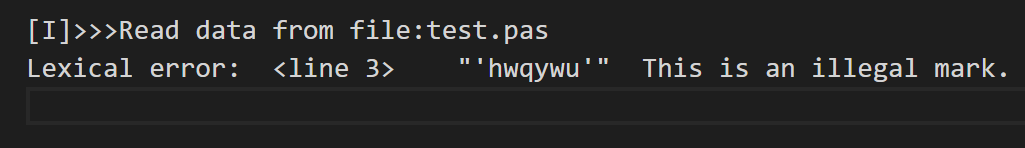
\includegraphics{C:/acm/coding/Project1/test.assets/image-20210509224823221.png}
    \caption{}
    \end{figure}
  \end{enumerate}
\end{enumerate}

\hypertarget{header-n286}{%
\paragraph{(2)语法分析}\label{header-n286}}

\begin{enumerate}
\def\labelenumi{\arabic{enumi}.}
\item
  括号不匹配

  \begin{enumerate}
  \def\labelenumii{\arabic{enumii}.}
  \item
    测试用例

\begin{Shaded}
\begin{Highlighting}[]
\KeywordTok{program}\NormalTok{ testLex(input, output;
}
\NormalTok{var
}
\NormalTok{	i, j, tmp, size: }\DataTypeTok{integer}\NormalTok{;
}
\NormalTok{	list:}\KeywordTok{array}\NormalTok{[}\DecValTok{0}\NormalTok{..}\DecValTok{1000}\NormalTok{] }\KeywordTok{of} \DataTypeTok{integer}\NormalTok{;
}
\KeywordTok{begin}

    \KeywordTok{for}\NormalTok{ i := }\DecValTok{1} \KeywordTok{to}\NormalTok{ size}\DecValTok{-1}\NormalTok{ do
}
	\KeywordTok{for}\NormalTok{ j := }\DecValTok{1} \KeywordTok{to}\NormalTok{ i do
}
	    \KeywordTok{if}\NormalTok{ list[j] > list[j+}\DecValTok{1}\NormalTok{] then
}
	    \KeywordTok{begin}

\NormalTok{		    tmp := list[j];
}
\NormalTok{		    list[j] := list[j+}\DecValTok{1}\NormalTok{];
}
\NormalTok{		    list [j+}\DecValTok{1}\NormalTok{] := tmp;
}
	    \KeywordTok{end}\NormalTok{;
}


    \KeywordTok{for}\NormalTok{ i :=}\DecValTok{1} \KeywordTok{to}\NormalTok{ size do
}
	\KeywordTok{write}\NormalTok{(list[i])
}
\KeywordTok{end}\NormalTok{.}
\end{Highlighting}
\end{Shaded}
  \item
    预期结果

    上述代码的词法分析结果正常,但在第一行出现了括号未匹配的问题
    \textbf{(input,
    output;},由语法分析部分报错,要求输出结果声明为语法分析,并给出错误行号为\textbf{1},输出预测的错误内容。
  \item
    测试结果及分析

    \begin{figure}
    \centering
    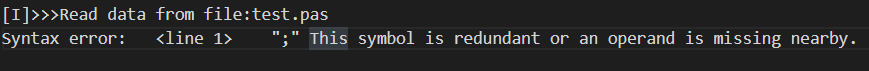
\includegraphics{C:/acm/coding/Project1/test.assets/image-20210511213831174.png}
    \caption{}
    \end{figure}
  \end{enumerate}
\item
  操作数缺失

  \begin{enumerate}
  \def\labelenumii{\arabic{enumii}.}
  \item
    测试用例

\begin{Shaded}
\begin{Highlighting}[]
\KeywordTok{program}\NormalTok{ testLex(input, output);
}
\NormalTok{var
}
\NormalTok{	i, j, tmp, size: }\DataTypeTok{integer}\NormalTok{;
}
\NormalTok{	list:}\KeywordTok{array}\NormalTok{[}\DecValTok{0}\NormalTok{..}\DecValTok{1000}\NormalTok{] }\KeywordTok{of} \DataTypeTok{integer}\NormalTok{;
}
\KeywordTok{begin}

    \KeywordTok{for}\NormalTok{ i := }\KeywordTok{to}\NormalTok{ size}\DecValTok{-1}\NormalTok{ do
}
	\KeywordTok{for}\NormalTok{ j := }\DecValTok{1} \KeywordTok{to}\NormalTok{ i do
}
	    \KeywordTok{if}\NormalTok{ list[j] > list[j+}\DecValTok{1}\NormalTok{] then
}
	    \KeywordTok{begin}

\NormalTok{		    tmp := list[j];
}
\NormalTok{		    list[j] := list[j+}\DecValTok{1}\NormalTok{];
}
\NormalTok{		    list [j+}\DecValTok{1}\NormalTok{] := tmp;
}
	    \KeywordTok{end}\NormalTok{;
}


    \KeywordTok{for}\NormalTok{ i :=}\DecValTok{1} \KeywordTok{to}\NormalTok{ size do
}
	\KeywordTok{write}\NormalTok{(list[i])
}
\KeywordTok{end}\NormalTok{.}
\end{Highlighting}
\end{Shaded}
  \item
    预期结果

    上述代码在第六行本应是\textbf{for i := 1 to size-1
    do},但实际却缺少了操作数1,但语法分析并不能准确识别这里属于操作数缺失,而只能识别出这里出现了错误,故在报错信息中会给出错误类别为\textbf{语法错误},给出错误行号,并给出识别到错误时当前识别到的字符以及预测该错误具体可能是什么,但未必准确。
  \item
    测试结果及分析

    \begin{figure}
    \centering
    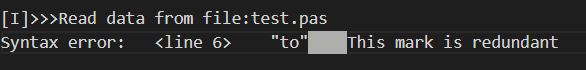
\includegraphics{C:/acm/coding/Project1/test.assets/image-20210511214117287.png}
    \caption{}
    \end{figure}
  \end{enumerate}
\item
  符号冗余

  \begin{enumerate}
  \def\labelenumii{\arabic{enumii}.}
  \item
    测试用例

\begin{Shaded}
\begin{Highlighting}[]
\KeywordTok{program}\NormalTok{ testLex(input, output);
}
\NormalTok{var
}
\NormalTok{	i,, j, tmp, size: }\DataTypeTok{integer}\NormalTok{;
}
\NormalTok{	list:}\KeywordTok{array}\NormalTok{[}\DecValTok{0}\NormalTok{..}\DecValTok{1000}\NormalTok{] }\KeywordTok{of} \DataTypeTok{integer}\NormalTok{;
}
\KeywordTok{begin}

    \KeywordTok{for}\NormalTok{ i := }\DecValTok{1} \KeywordTok{to}\NormalTok{ size}\DecValTok{-1}\NormalTok{ do
}
	\KeywordTok{for}\NormalTok{ j := }\DecValTok{1} \KeywordTok{to}\NormalTok{ i do
}
	    \KeywordTok{if}\NormalTok{ list[j] > list[j+}\DecValTok{1}\NormalTok{] then
}
	    \KeywordTok{begin}

\NormalTok{		    tmp := list[j];
}
\NormalTok{		    list[j] := list[j+}\DecValTok{1}\NormalTok{];
}
\NormalTok{		    list [j+}\DecValTok{1}\NormalTok{] := tmp;
}
	    \KeywordTok{end}\NormalTok{;
}


    \KeywordTok{for}\NormalTok{ i :=}\DecValTok{1} \KeywordTok{to}\NormalTok{ size do
}
	\KeywordTok{write}\NormalTok{(list[i])
}
\KeywordTok{end}\NormalTok{.}
\end{Highlighting}
\end{Shaded}
  \item
    预期结果

    该测试样例在词法上没有问题,但在语法分析时会发现第三行出现了重复的两个\textbf{","},语法分析会识别出该错误,并报告语法分析异常,给出出错行号为\textbf{3},错误类型为符号冗余,并停止程序的继续执行。
  \item
    测试结果及分析

    \begin{figure}
    \centering
    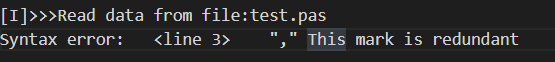
\includegraphics{C:/acm/coding/Project1/test.assets/image-20210511214313718.png}
    \caption{}
    \end{figure}
  \end{enumerate}
\item
  符号缺失

  \begin{enumerate}
  \def\labelenumii{\arabic{enumii}.}
  \item
    测试用例

\begin{Shaded}
\begin{Highlighting}[]
\KeywordTok{program}\NormalTok{ testLex(input, output);
}
\NormalTok{var
}
\NormalTok{	i, j, tmp, size: integer
}
\NormalTok{	list:}\KeywordTok{array}\NormalTok{[}\DecValTok{0}\NormalTok{..}\DecValTok{1000}\NormalTok{] }\KeywordTok{of} \DataTypeTok{integer}\NormalTok{;
}
\KeywordTok{begin}

    \KeywordTok{for}\NormalTok{ i := }\DecValTok{1} \KeywordTok{to}\NormalTok{ size}\DecValTok{-1}\NormalTok{ do
}
	\KeywordTok{for}\NormalTok{ j := }\DecValTok{1} \KeywordTok{to}\NormalTok{ i do
}
	    \KeywordTok{if}\NormalTok{ list[j] > list[j+}\DecValTok{1}\NormalTok{] then
}
	    \KeywordTok{begin}

\NormalTok{		    tmp := list[j];
}
\NormalTok{		    list[j] := list[j+}\DecValTok{1}\NormalTok{];
}
\NormalTok{		    list [j+}\DecValTok{1}\NormalTok{] := tmp;
}
	    \KeywordTok{end}\NormalTok{;
}


    \KeywordTok{for}\NormalTok{ i :=}\DecValTok{1} \KeywordTok{to}\NormalTok{ size do
}
	\KeywordTok{write}\NormalTok{(list[i])
}
\KeywordTok{end}\NormalTok{.}
\end{Highlighting}
\end{Shaded}
  \item
    预期结果

    在\textbf{第3行}缺少了结束的\textbf{;},语法分析报错,输出错误类型语法错误,错误行号3,错误内容为符号缺失。
  \item
    测试结果及分析

    \begin{figure}
    \centering
    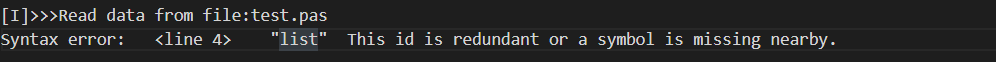
\includegraphics{C:/acm/coding/Project1/test.assets/image-20210511214433480.png}
    \caption{}
    \end{figure}

    在实际测试时,发现错误行号输出并不是\textbf{3,而是4},因为在语法分析的错误分析时,并不能完全准确的识别出错误的发生地点,而只能给出发生了语法错误时正在识别的那个符号的位置,在发生\textbf{``;''}缺失的那一行当时语法分析并没有立即识别出错误,而在下一行才开始发现发生了语法错误,所以发生了错误报错行号与实际错误行号不一致的情况。
  \end{enumerate}
\end{enumerate}

\hypertarget{header-n287}{%
\paragraph{(3)语义分析 }\label{header-n287}}

\begin{enumerate}
\def\labelenumi{\arabic{enumi}.}
\item
  常量重复定义

  测试用例:

\begin{Shaded}
\begin{Highlighting}[]
\KeywordTok{program}\NormalTok{ test;}
\KeywordTok{const}
\NormalTok{    a=}\DecValTok{1}\NormalTok{;}
\NormalTok{    a=}\DecValTok{1.0}\NormalTok{;}
\KeywordTok{begin}
\KeywordTok{end}\NormalTok{.}
\end{Highlighting}
\end{Shaded}

  预期结果:

  \textbf{'a=1.0'}处报告重复定义错误。

  测试结果:

  \begin{figure}
  \centering
  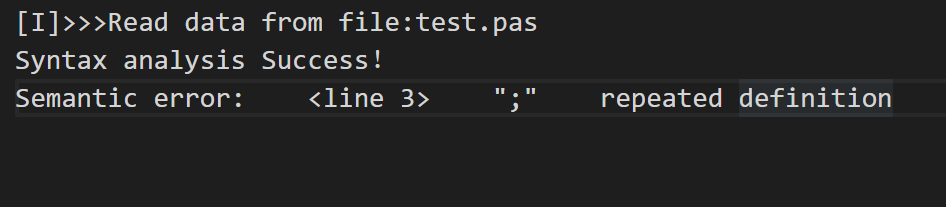
\includegraphics{C:/acm/coding/Project1/test.assets/image-20210509154828153.png}
  \caption{image-20210509154828153}
  \end{figure}
\item
  变量重复定义
\end{enumerate}

测试用例:

\begin{Shaded}
\begin{Highlighting}[]
  \KeywordTok{program}\NormalTok{ test;}
  \KeywordTok{var}
\NormalTok{  	a:}\DataTypeTok{integer}\NormalTok{;}
\NormalTok{  	a:}\DataTypeTok{real}\NormalTok{;}
  \KeywordTok{begin}
  	
  \KeywordTok{end}\NormalTok{.}
\end{Highlighting}
\end{Shaded}

预期结果:

\textbf{'a:real'}处报告重复定义错误;

测试结果:

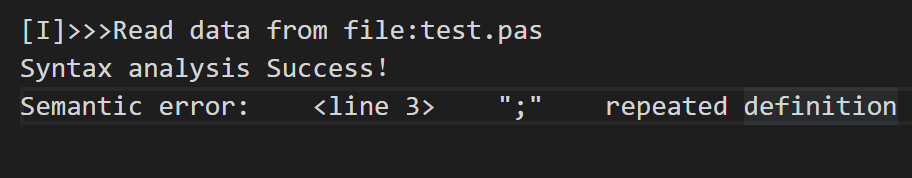
\includegraphics{C:/acm/coding/Project1/语义分析测试.assets/image-20210509185024679.png}

\begin{enumerate}
\def\labelenumi{\arabic{enumi}.}
\item
  常量被赋值
\end{enumerate}

测试用例:

\begin{Shaded}
\begin{Highlighting}[]
  
  \KeywordTok{program}\NormalTok{ a;}
  \KeywordTok{var}
\NormalTok{      b:}\DataTypeTok{integer}\NormalTok{;}
  \KeywordTok{procedure}\NormalTok{ gcd(}\KeywordTok{var}\NormalTok{ a:}\DataTypeTok{integer}\NormalTok{);}
  \KeywordTok{const}
\NormalTok{      b=}\DecValTok{1}\NormalTok{;}
  \KeywordTok{begin}
\NormalTok{      b:=a;}
  \KeywordTok{end}\NormalTok{;}
  \KeywordTok{begin}
\NormalTok{      gcd(b);}
  \KeywordTok{end}\NormalTok{.}
  
\end{Highlighting}
\end{Shaded}

预期结果:

\textbf{'b:=a'}处报错。

测试结果:

\begin{figure}
\centering
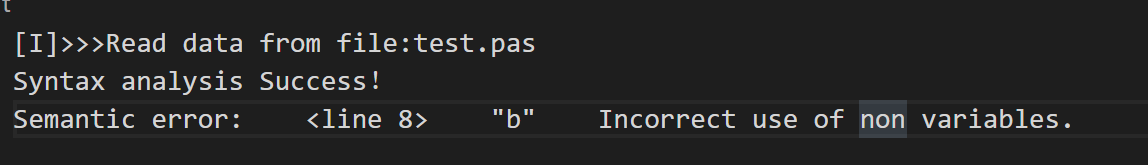
\includegraphics{C:/acm/coding/Project1/test.assets/image-20210509192405852.png}
\caption{image-20210509192405852}
\end{figure}

4.使用未定义的常量

测试用例:

\begin{Shaded}
\begin{Highlighting}[]
\KeywordTok{program}\NormalTok{ test(input,output);   }
\KeywordTok{begin}
\NormalTok{	a:=}\DecValTok{1}\NormalTok{;}
\KeywordTok{end}\NormalTok{.}
\end{Highlighting}
\end{Shaded}

预期结果:

\textbf{'a:=1'}处报错

测试结果:

\begin{figure}
\centering
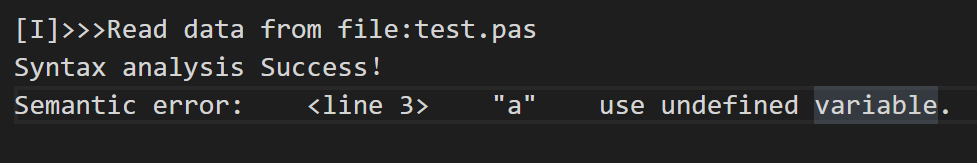
\includegraphics{C:/acm/coding/Project1/test.assets/image-20210509192636999.png}
\caption{image-20210509192636999}
\end{figure}

5 if中判断条件的类型错误

测试用例:

\begin{Shaded}
\begin{Highlighting}[]
\KeywordTok{program}\NormalTok{ test(input,output);}
\KeywordTok{var}\NormalTok{ a,b:}\DataTypeTok{integer}\NormalTok{;  }
\NormalTok{    c:}\DataTypeTok{boolean}\NormalTok{;  }
\NormalTok{    d:}\DataTypeTok{real}\NormalTok{;  }
\NormalTok{    e:}\DataTypeTok{char}\NormalTok{;  }
\KeywordTok{begin}  
\NormalTok{    a:=}\DecValTok{1}\NormalTok{;   }
    \KeywordTok{if}\NormalTok{ d }\KeywordTok{then}  
        \KeywordTok{begin}  
\NormalTok{            a:=a+}\DecValTok{1}\NormalTok{;  }
        \KeywordTok{end}  
    \KeywordTok{else}  
        \KeywordTok{begin}  
\NormalTok{            a:=a+}\DecValTok{10}\NormalTok{;    }
        \KeywordTok{end}\NormalTok{;}
\KeywordTok{end}\NormalTok{. }
\end{Highlighting}
\end{Shaded}

预期结果:

\textbf{'if c then'}处报错

测试结果:

\begin{figure}
\centering
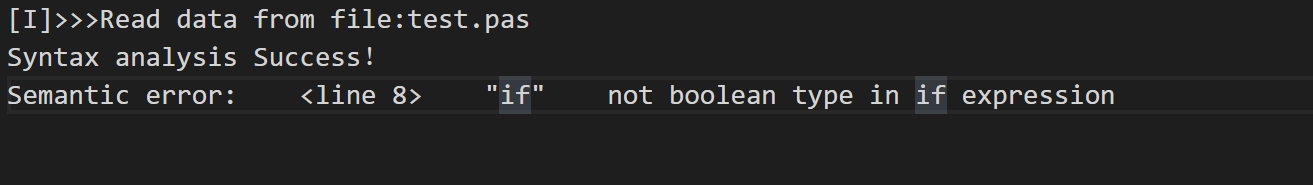
\includegraphics{C:/acm/coding/Project1/test.assets/image-20210509193115980.png}
\caption{image-20210509193115980}
\end{figure}

\begin{enumerate}
\def\labelenumi{\arabic{enumi}.}
\item
  for中循环变量类型错误

  测试用例:

\begin{Shaded}
\begin{Highlighting}[]
\NormalTok{program test(input,output);  }
\NormalTok{var a,b:integer;  }
\NormalTok{    c:}\DataTypeTok{char}\NormalTok{;  }
\NormalTok{begin  }
\ControlFlowTok{for}\NormalTok{ a:=}\DecValTok{6}\NormalTok{ to }\DecValTok{1+3} \ControlFlowTok{do}  \CommentTok{//正确}
\NormalTok{    write(b);  }
\ControlFlowTok{for}\NormalTok{ a:=c to a+b }\ControlFlowTok{do} \CommentTok{//start表达式不是integer类型  }
\NormalTok{    write(a);  }
\NormalTok{end. }
\end{Highlighting}
\end{Shaded}

  预期结果:

  \textbf{'a:=c'}处报错

  测试结果:

  \begin{figure}
  \centering
  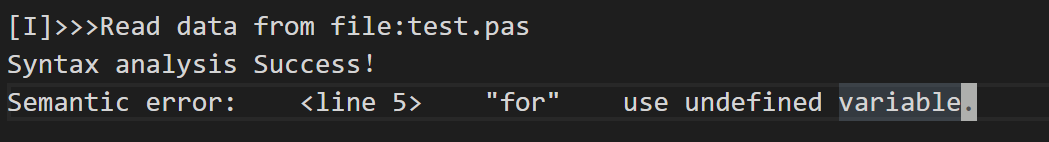
\includegraphics{C:/acm/coding/Project1/test.assets/image-20210509204233548.png}
  \caption{image-20210509204233548}
  \end{figure}

  \begin{enumerate}
  \def\labelenumii{\arabic{enumii}.}
  \item
    数组定义上限小于下限
  \end{enumerate}

  测试样例:

\begin{Shaded}
\begin{Highlighting}[]
\KeywordTok{program}\NormalTok{ test(input,output);  }
\KeywordTok{var}\NormalTok{ b:}\KeywordTok{array}\NormalTok{[}\DecValTok{5}\NormalTok{..}\DecValTok{10}\NormalTok{] }\KeywordTok{of} \DataTypeTok{integer}\NormalTok{;}
\NormalTok{    a:}\KeywordTok{array}\NormalTok{[}\DecValTok{10}\NormalTok{..}\DecValTok{5}\NormalTok{] }\KeywordTok{of} \DataTypeTok{integer}\NormalTok{;}
\KeywordTok{begin}  
  
\KeywordTok{end}\NormalTok{.  }
\end{Highlighting}
\end{Shaded}

  预期结果:

  \textbf{'10..5'}处报错

  测试结果:

  \begin{figure}
  \centering
  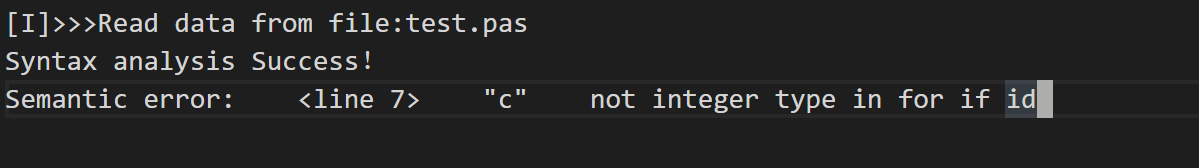
\includegraphics{C:/acm/coding/Project1/test.assets/image-20210509214136051.png}
  \caption{image-20210509214136051}
  \end{figure}

  \begin{enumerate}
  \def\labelenumii{\arabic{enumii}.}
  \item
    数组使用类型不是int

    测试样例:

\begin{Shaded}
\begin{Highlighting}[]
\KeywordTok{program}\NormalTok{ test(input,output);  }
\KeywordTok{const}\NormalTok{ e=}\DecValTok{10}\NormalTok{;  }
\NormalTok{      f=}\DecValTok{20}\NormalTok{;  }
\KeywordTok{var}\NormalTok{ a: }\KeywordTok{array}\NormalTok{[}\DecValTok{0}\NormalTok{..}\DecValTok{5}\NormalTok{,}\DecValTok{6}\NormalTok{..}\DecValTok{10}\NormalTok{,}\DecValTok{11}\NormalTok{..}\DecValTok{15}\NormalTok{] }\KeywordTok{of} \DataTypeTok{integer}\NormalTok{;  }
\NormalTok{    b,c: }\DataTypeTok{integer}\NormalTok{;  }
\NormalTok{    d: }\DataTypeTok{char}\NormalTok{;  }
\KeywordTok{begin}  
\NormalTok{    a[d,b>c,b+c]:=b; }
\KeywordTok{end}\NormalTok{. }
\end{Highlighting}
\end{Shaded}

    预期结果:

    \textbf{'b\textgreater{}c'}处报错

    测试结果:

    \begin{figure}
    \centering
    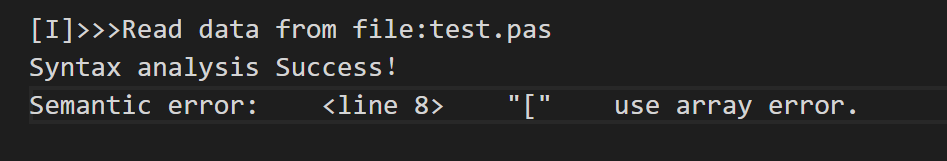
\includegraphics{C:/acm/coding/Project1/test.assets/image-20210509214724675.png}
    \caption{image-20210509214724675}
    \end{figure}
  \item
    数组使用维数错误
  \end{enumerate}

  测试样例:

\begin{Shaded}
\begin{Highlighting}[]
\KeywordTok{program}\NormalTok{ test(input,output);  }
\KeywordTok{var}\NormalTok{ a: }\KeywordTok{array}\NormalTok{[}\DecValTok{0}\NormalTok{..}\DecValTok{5}\NormalTok{,}\DecValTok{6}\NormalTok{..}\DecValTok{10}\NormalTok{,}\DecValTok{11}\NormalTok{..}\DecValTok{15}\NormalTok{] }\KeywordTok{of} \DataTypeTok{integer}\NormalTok{;  }
\NormalTok{    b: }\DataTypeTok{integer}\NormalTok{;  }
\KeywordTok{begin}  
\NormalTok{    a[}\DecValTok{0}\NormalTok{]:=b;  }
\NormalTok{    b:=a[}\DecValTok{0}\NormalTok{, }\DecValTok{6}\NormalTok{];  }
\NormalTok{    a[}\DecValTok{0}\NormalTok{, }\DecValTok{6}\NormalTok{, }\DecValTok{11}\NormalTok{]:=b;  }
\NormalTok{    b:=a[}\DecValTok{0}\NormalTok{, }\DecValTok{6}\NormalTok{, }\DecValTok{11}\NormalTok{, }\DecValTok{16}\NormalTok{];  }
\KeywordTok{end}\NormalTok{.  }
\end{Highlighting}
\end{Shaded}

  预期结果:

  \textbf{'a{[}0{]}:=6'}处报错

  测试结果:

  \begin{figure}
  \centering
  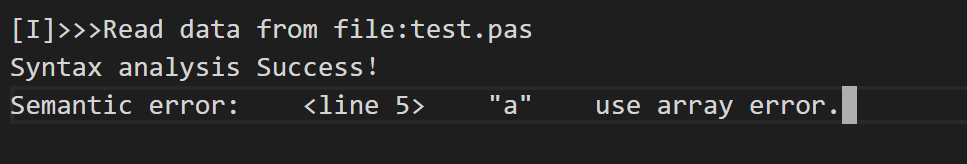
\includegraphics{C:/acm/coding/Project1/test.assets/image-20210509215844226.png}
  \caption{image-20210509215844226}
  \end{figure}

  \begin{enumerate}
  \def\labelenumii{\arabic{enumii}.}
  \item
    函数未定义使用错误
  \end{enumerate}

  测试样例:

\begin{Shaded}
\begin{Highlighting}[]
\KeywordTok{program}\NormalTok{ test(input,output);  }
\KeywordTok{const}\NormalTok{ f=}\DecValTok{5}\NormalTok{;  }
\KeywordTok{var}\NormalTok{ a,b:}\DataTypeTok{integer}\NormalTok{;  }
\NormalTok{    c:}\KeywordTok{array}\NormalTok{[}\DecValTok{1}\NormalTok{..}\DecValTok{5}\NormalTok{] }\KeywordTok{of} \DataTypeTok{integer}\NormalTok{;    }
\KeywordTok{begin}  
\NormalTok{    a:=fun(}\DecValTok{1}\NormalTok{);}
\KeywordTok{end}\NormalTok{.}
\end{Highlighting}
\end{Shaded}

  预期结果:

  \textbf{'fun(1)'}处报错

  测试结果:

  \begin{figure}
  \centering
  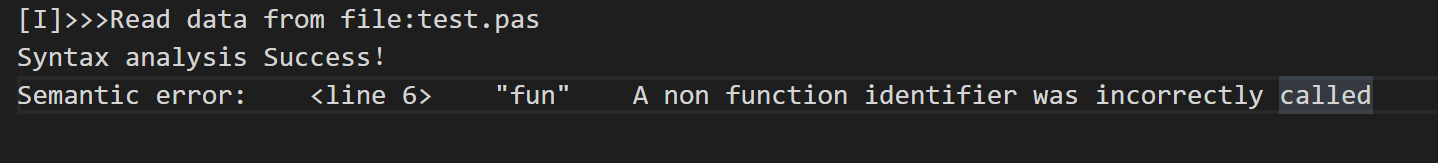
\includegraphics{C:/acm/coding/Project1/test.assets/image-20210509220803043.png}
  \caption{image-20210509220803043}
  \end{figure}

  11.函数调用参数类型错误

  测试样例:

\begin{Shaded}
\begin{Highlighting}[]
\KeywordTok{program}\NormalTok{ test(input,output);  }
\KeywordTok{const}\NormalTok{ h=}\DecValTok{5}\NormalTok{;  }
\KeywordTok{var}\NormalTok{ d:}\KeywordTok{array}\NormalTok{[}\DecValTok{1}\NormalTok{..}\DecValTok{5}\NormalTok{] }\KeywordTok{of} \DataTypeTok{integer}\NormalTok{;  }
\NormalTok{    e,f,g:}\DataTypeTok{integer}\NormalTok{; }
\NormalTok{	m:}\DataTypeTok{char}\NormalTok{; }
\KeywordTok{procedure}\NormalTok{ pro(}\KeywordTok{var}\NormalTok{ a,b,c:}\DataTypeTok{integer}\NormalTok{);}
\KeywordTok{begin}  
    \KeywordTok{if}\NormalTok{ a<=b }\KeywordTok{then}  
        \KeywordTok{if}\NormalTok{ b<=c }\KeywordTok{then}  
            \KeywordTok{write}\NormalTok{(}\DecValTok{1}\NormalTok{)   }
\KeywordTok{end}\NormalTok{;  }
\KeywordTok{begin} 
\NormalTok{    pro(d[}\DecValTok{1}\NormalTok{],d[}\DecValTok{2}\NormalTok{],d[}\DecValTok{3}\NormalTok{]);}
\NormalTok{	pro(m,e,f);}
\KeywordTok{end}\NormalTok{. }
\end{Highlighting}
\end{Shaded}

  预期结果:

  \textbf{'pro(m,e,f)'}处报错

  测试结果:

  \begin{figure}
  \centering
  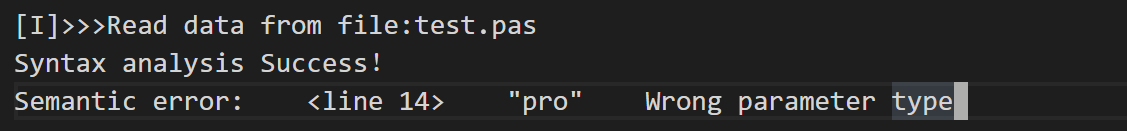
\includegraphics{C:/acm/coding/Project1/test.assets/image-20210509221946400.png}
  \caption{image-20210509221946400}
  \end{figure}

  12.函数参数数量错误

  测试用例:
\end{enumerate}

\begin{Shaded}
\begin{Highlighting}[]
\KeywordTok{program}\NormalTok{ test(input,output);  
}
\KeywordTok{const}\NormalTok{ h=}\DecValTok{5}\NormalTok{;  
}
\KeywordTok{var}\NormalTok{ d:}\KeywordTok{array}\NormalTok{[}\DecValTok{1}\NormalTok{..}\DecValTok{5}\NormalTok{] }\KeywordTok{of} \DataTypeTok{integer}\NormalTok{;  
}
\NormalTok{    e,f,g:}\DataTypeTok{integer}\NormalTok{; 
}
\NormalTok{	m:}\DataTypeTok{char}\NormalTok{; 
}
\KeywordTok{procedure}\NormalTok{ pro(}\KeywordTok{var}\NormalTok{ a,b,c,d:}\DataTypeTok{integer}\NormalTok{);
}
\KeywordTok{begin}  

    \KeywordTok{if}\NormalTok{ a<=b }\KeywordTok{then}  

        \KeywordTok{if}\NormalTok{ b<=c }\KeywordTok{then}  

            \KeywordTok{write}\NormalTok{(}\DecValTok{1}\NormalTok{)   
}
\KeywordTok{end}\NormalTok{;  
}
\KeywordTok{begin} 

\NormalTok{    pro(d[}\DecValTok{1}\NormalTok{],d[}\DecValTok{2}\NormalTok{],d[}\DecValTok{3}\NormalTok{]);
}
\KeywordTok{end}\NormalTok{. }
\end{Highlighting}
\end{Shaded}

预期结果:

\textbf{'pro(d{[}1{]},d{[}2{]},d{[}3{]})'}处报错

测试结果:

\begin{figure}
\centering
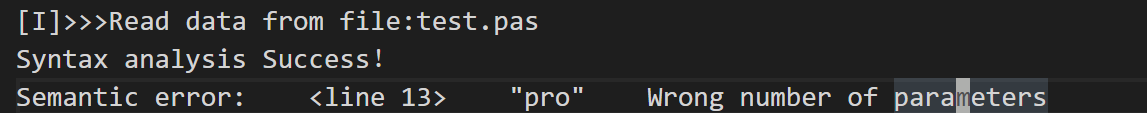
\includegraphics{C:/acm/coding/Project1/test.assets/image-20210509222412577.png}
\caption{image-20210509222412577}
\end{figure}

13.引用参数调用时使用非单个变量

测试用例:

\begin{Shaded}
\begin{Highlighting}[]


\KeywordTok{program}\NormalTok{ a;
}
\NormalTok{var
}
\NormalTok{    b:}\DataTypeTok{integer}\NormalTok{;
}
\KeywordTok{function}\NormalTok{ gcd(}\KeywordTok{var}\NormalTok{ a:}\DataTypeTok{integer}\NormalTok{):}\DataTypeTok{integer}\NormalTok{;
}
\KeywordTok{begin}

    \KeywordTok{if}\NormalTok{ a=}\DecValTok{0} \KeywordTok{then}\NormalTok{ gcd:=}\DecValTok{1}

    \KeywordTok{else}\NormalTok{ gcd:=a*gcd(a);
}
\KeywordTok{end}\NormalTok{;
}
\KeywordTok{begin}

\NormalTok{    gcd(b}\DecValTok{-1}\NormalTok{);
}
\KeywordTok{end}\NormalTok{.
}
\end{Highlighting}
\end{Shaded}

预期结果:

\textbf{'gcd(b-1)'}处报错

测试结果:

\begin{figure}
\centering
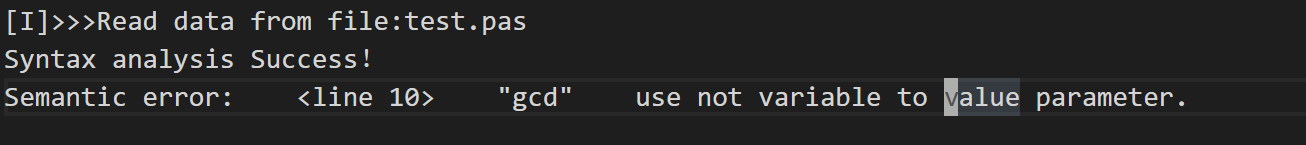
\includegraphics{C:/acm/coding/Project1/test.assets/image-20210509222943638.png}
\caption{image-20210509222943638}
\end{figure}

\hypertarget{header-n399}{%
\subsection{代码生成测试}\label{header-n399}}

\begin{enumerate}
\def\labelenumi{\arabic{enumi}.}
\item
  基础功能测试
\end{enumerate}

测试样例

\begin{Shaded}
\begin{Highlighting}[]
\KeywordTok{program}\NormalTok{ a;
}
\KeywordTok{const} 

\NormalTok{    maxN=}\DecValTok{200005}\NormalTok{;
}
\NormalTok{    a=}\DecValTok{123.0}\NormalTok{;
}
\NormalTok{    c=}\StringTok{'a'}\NormalTok{;
}
\NormalTok{    d=-}\DecValTok{1325}\NormalTok{;
}
\NormalTok{    e=+}\DecValTok{3253}\NormalTok{;
}
\NormalTok{var
}
\NormalTok{    f,g,k,b:}\DataTypeTok{integer}\NormalTok{;
}
\NormalTok{      h,i:}\DataTypeTok{char}\NormalTok{;
}
\NormalTok{    dfds,c2,g3:}\DataTypeTok{boolean}\NormalTok{;
}
\NormalTok{    dfsge1312,d13,reww:}\DataTypeTok{real}\NormalTok{;
}
 \KeywordTok{begin}

\NormalTok{    d13:=(g+f)*k / b;
}
\NormalTok{	c2:=h>i;
}
\NormalTok{	reww:=(dfsge1312+reww)-k+b }\KeywordTok{mod}\NormalTok{ (f+g)
}
    

 \KeywordTok{end}\NormalTok{.}
\end{Highlighting}
\end{Shaded}

测试结果:

\begin{Shaded}
\begin{Highlighting}[]
\PreprocessorTok{#include }\ImportTok{<stdio.h>}\PreprocessorTok{
}


\DataTypeTok{const} \DataTypeTok{short}\NormalTok{ maxn = }\DecValTok{200005}\NormalTok{;
}
\DataTypeTok{const} \DataTypeTok{float}\NormalTok{ a = }\FloatTok{123.0}\NormalTok{;
}
\DataTypeTok{const} \DataTypeTok{char}\NormalTok{ c = }\CharTok{'a'}\NormalTok{;
}
\DataTypeTok{const} \DataTypeTok{short}\NormalTok{ d = }\DecValTok{-1325}\NormalTok{;
}
\DataTypeTok{const} \DataTypeTok{short}\NormalTok{ e = +}\DecValTok{3253}\NormalTok{;
}
\DataTypeTok{short}\NormalTok{ f, g, k, b;
}
\DataTypeTok{char}\NormalTok{ h, i;
}
\DataTypeTok{bool}\NormalTok{ dfds, c2, g3;
}
\DataTypeTok{float}\NormalTok{ dfsge1312, d13, reww;
}
\DataTypeTok{int}\NormalTok{ main()
}
\NormalTok{\{
}
\NormalTok{    d13 = (g + f) * k / (}\DataTypeTok{float}\NormalTok{)b;
}
\NormalTok{    c2 = h > i;
}
\NormalTok{    reww = (dfsge1312 + reww) - k + b % (f + g);
}
    \ControlFlowTok{return} \DecValTok{0}\NormalTok{;
}
\NormalTok{\}}
\end{Highlighting}
\end{Shaded}

\begin{enumerate}
\def\labelenumi{\arabic{enumi}.}
\item
  数组测试
\end{enumerate}

测试样例:

本样例主要测试的是能否将数组做出正确的处理,

由于C语言与pascal语言对于数组定义的不同,转换时需要减去下标

\begin{Shaded}
\begin{Highlighting}[]
\KeywordTok{program}\NormalTok{ a;
}
\KeywordTok{var} 

\NormalTok{    c :}\KeywordTok{array}\NormalTok{ [}\DecValTok{105}\NormalTok{..}\DecValTok{1000}\NormalTok{] }\KeywordTok{of} \DataTypeTok{integer}\NormalTok{;
}
\NormalTok{    d :}\KeywordTok{array}\NormalTok{ [}\DecValTok{34}\NormalTok{..}\DecValTok{500}\NormalTok{,}\DecValTok{78}\NormalTok{..}\DecValTok{897}\NormalTok{] }\KeywordTok{of} \DataTypeTok{integer}\NormalTok{;
}
 \KeywordTok{function}\NormalTok{ gcd(a,b:}\DataTypeTok{integer}\NormalTok{):}\DataTypeTok{integer}\NormalTok{;
}
\NormalTok{ var
}
\NormalTok{    c :}\KeywordTok{array}\NormalTok{ [}\DecValTok{105}\NormalTok{..}\DecValTok{1000}\NormalTok{,}\DecValTok{73}\NormalTok{..}\DecValTok{100}\NormalTok{] }\KeywordTok{of} \DataTypeTok{integer}\NormalTok{;
}
\NormalTok{     e :}\KeywordTok{array}\NormalTok{ [}\DecValTok{105}\NormalTok{..}\DecValTok{1000}\NormalTok{] }\KeywordTok{of} \DataTypeTok{integer}\NormalTok{;
}
\NormalTok{     f :}\KeywordTok{array}\NormalTok{ [}\DecValTok{34}\NormalTok{..}\DecValTok{500}\NormalTok{,}\DecValTok{78}\NormalTok{..}\DecValTok{897}\NormalTok{] }\KeywordTok{of} \DataTypeTok{integer}\NormalTok{;
}
        \KeywordTok{begin} 

         \KeywordTok{read}\NormalTok{(e[}\DecValTok{768}\NormalTok{]);
}
        \KeywordTok{write}\NormalTok{(f[}\DecValTok{54}\NormalTok{,}\DecValTok{97}\NormalTok{]);
}
        \KeywordTok{read}\NormalTok{(c[}\DecValTok{768}\NormalTok{,}\DecValTok{79}\NormalTok{]);
}
        \KeywordTok{write}\NormalTok{(d[}\DecValTok{54}\NormalTok{,}\DecValTok{97}\NormalTok{]);
}
        \KeywordTok{if}\NormalTok{ b=}\DecValTok{0} \KeywordTok{then}\NormalTok{ gcd:=a
}
        \KeywordTok{else}\NormalTok{ gcd:=gcd(b, a }\KeywordTok{mod}\NormalTok{ b)
}
        \KeywordTok{end}\NormalTok{;
}
 \KeywordTok{begin}

    \KeywordTok{write}\NormalTok{(c[d[}\DecValTok{32}\NormalTok{,}\DecValTok{47}\NormalTok{]],d[}\DecValTok{45}\NormalTok{,}\DecValTok{79}\NormalTok{]);
}
 \KeywordTok{end}\NormalTok{.}
\end{Highlighting}
\end{Shaded}

测试结果:

\begin{Shaded}
\begin{Highlighting}[]
\PreprocessorTok{#include }\ImportTok{<stdio.h>}\PreprocessorTok{
}


\DataTypeTok{short}\NormalTok{ c[}\DecValTok{896}\NormalTok{];
}
\DataTypeTok{short}\NormalTok{ d[}\DecValTok{467}\NormalTok{][}\DecValTok{820}\NormalTok{];
}
\DataTypeTok{short}\NormalTok{ gcd(}\DataTypeTok{short}\NormalTok{ a, }\DataTypeTok{short}\NormalTok{ b)
}
\NormalTok{\{
}
    \DataTypeTok{short}\NormalTok{ gcd_returnVal;
}
    \DataTypeTok{short}\NormalTok{ c[}\DecValTok{896}\NormalTok{][}\DecValTok{28}\NormalTok{];
}
    \DataTypeTok{short}\NormalTok{ e[}\DecValTok{896}\NormalTok{];
}
    \DataTypeTok{short}\NormalTok{ f[}\DecValTok{467}\NormalTok{][}\DecValTok{820}\NormalTok{];
}
\NormalTok{    scanf(}\StringTok{"}\SpecialCharTok{%hd}\StringTok{"}\NormalTok{, &e[}\DecValTok{768}\NormalTok{ - }\DecValTok{105}\NormalTok{]);
}
\NormalTok{    printf(}\StringTok{"}\SpecialCharTok{%hd}\StringTok{"}\NormalTok{, f[}\DecValTok{54}\NormalTok{ - }\DecValTok{34}\NormalTok{][}\DecValTok{97}\NormalTok{ - }\DecValTok{78}\NormalTok{]);
}
\NormalTok{    scanf(}\StringTok{"}\SpecialCharTok{%hd}\StringTok{"}\NormalTok{, &c[}\DecValTok{768}\NormalTok{ - }\DecValTok{105}\NormalTok{][}\DecValTok{79}\NormalTok{ - }\DecValTok{73}\NormalTok{]);
}
\NormalTok{    printf(}\StringTok{"}\SpecialCharTok{%hd}\StringTok{"}\NormalTok{, d[}\DecValTok{54}\NormalTok{ - }\DecValTok{34}\NormalTok{][}\DecValTok{97}\NormalTok{ - }\DecValTok{78}\NormalTok{]);
}
    \ControlFlowTok{if}\NormalTok{ (b == }\DecValTok{0}\NormalTok{)
}
\NormalTok{        gcd_returnVal = a;
}
\NormalTok{    else
}
\NormalTok{        gcd_returnVal = gcd(b, a % b);
}
    \ControlFlowTok{return}\NormalTok{ gcd_returnVal;
}
\NormalTok{\}
}
\DataTypeTok{int}\NormalTok{ main()
}
\NormalTok{\{
}
\NormalTok{    printf(}\StringTok{"}\SpecialCharTok{%hd}\StringTok{ }\SpecialCharTok{%hd}\StringTok{"}\NormalTok{, c[d[}\DecValTok{32}\NormalTok{ - }\DecValTok{34}\NormalTok{][}\DecValTok{47}\NormalTok{ - }\DecValTok{78}\NormalTok{] - }\DecValTok{105}\NormalTok{], d[}\DecValTok{45}\NormalTok{ - }\DecValTok{34}\NormalTok{][}\DecValTok{79}\NormalTok{ - }\DecValTok{78}\NormalTok{]);
}
    \ControlFlowTok{return} \DecValTok{0}\NormalTok{;
}
\NormalTok{\}
}
\end{Highlighting}
\end{Shaded}

\begin{enumerate}
\def\labelenumi{\arabic{enumi}.}
\item
  递归测试:
\end{enumerate}

测试样例:

该样例主要目的为测试是否能够正确应对函数递归的情况,

代码的含义为计算两个数的最大公约数

\begin{Shaded}
\begin{Highlighting}[]
\KeywordTok{program}\NormalTok{ example(input,output);
}
    \KeywordTok{var}\NormalTok{ x,y:}\DataTypeTok{integer}\NormalTok{;
}
    \KeywordTok{function}\NormalTok{ gcd(a,b:}\DataTypeTok{integer}\NormalTok{):}\DataTypeTok{integer}\NormalTok{;
}
    \KeywordTok{var}\NormalTok{ d:}\DataTypeTok{integer}\NormalTok{;
}
        \KeywordTok{begin} 

            \KeywordTok{if}\NormalTok{ b=}\DecValTok{0} \KeywordTok{then}\NormalTok{ gcd:=a
}
            \KeywordTok{else}\NormalTok{ gcd:=b;
}
\NormalTok{            gcd:=}\DecValTok{1}\NormalTok{;
}
\NormalTok{            d:=gcd;
}
        \KeywordTok{end}\NormalTok{;
}
    \KeywordTok{begin}

        \KeywordTok{read}\NormalTok{(x, y);
}
        \KeywordTok{write}\NormalTok{(gcd(x, y))
}
    \KeywordTok{end}\NormalTok{.}
\end{Highlighting}
\end{Shaded}

测试结果:

\begin{Shaded}
\begin{Highlighting}[]
\PreprocessorTok{#include }\ImportTok{<stdio.h>}\PreprocessorTok{
}


\DataTypeTok{short}\NormalTok{ x, y;
}
\DataTypeTok{short}\NormalTok{ gcd(}\DataTypeTok{short}\NormalTok{ a, }\DataTypeTok{short}\NormalTok{ b)
}
\NormalTok{\{
}
    \DataTypeTok{short}\NormalTok{ gcd_returnVal;
}
    \DataTypeTok{short}\NormalTok{ d;
}
    \ControlFlowTok{if}\NormalTok{ (b == }\DecValTok{0}\NormalTok{)
}
\NormalTok{        gcd_returnVal = a;
}
\NormalTok{    else
}
\NormalTok{        gcd_returnVal = b;
}
\NormalTok{    gcd_returnVal = }\DecValTok{1}\NormalTok{;
}
\NormalTok{    d = gcd_returnVal;
}
    \ControlFlowTok{return}\NormalTok{ gcd_returnVal;
}
\NormalTok{\}
}
\DataTypeTok{int}\NormalTok{ main()
}
\NormalTok{\{
}
\NormalTok{    scanf(}\StringTok{"%hd %hd"}\NormalTok{, &x, &y);
}
\NormalTok{    printf(}\StringTok{"%hd"}\NormalTok{, gcd(x, y));
}
    \ControlFlowTok{return} \DecValTok{0}\NormalTok{;
}
\NormalTok{\}
}
\end{Highlighting}
\end{Shaded}

\begin{enumerate}
\def\labelenumi{\arabic{enumi}.}
\item
  快排测试
\end{enumerate}

测试样例:

该样例为快速排序算法

\begin{Shaded}
\begin{Highlighting}[]
\KeywordTok{program}\NormalTok{ qsort(input,output);
}
\NormalTok{var
}
\NormalTok{	n,i:}\DataTypeTok{integer}\NormalTok{;
}
\NormalTok{	list:}\KeywordTok{array}\NormalTok{[}\DecValTok{0}\NormalTok{..}\DecValTok{1000}\NormalTok{] }\KeywordTok{of} \DataTypeTok{integer}\NormalTok{;
}
\NormalTok{	c:}\DataTypeTok{char}\NormalTok{;
}
\KeywordTok{procedure}\NormalTok{ qsort(low, high:}\DataTypeTok{integer}\NormalTok{);
}
\NormalTok{var
}
\NormalTok{	l,h,m:}\DataTypeTok{integer}\NormalTok{;
}
\NormalTok{	i,j:}\DataTypeTok{integer}\NormalTok{;
}
\NormalTok{	temp:}\DataTypeTok{integer}\NormalTok{;
}
\NormalTok{	flag:}\DataTypeTok{integer}\NormalTok{;
}
\KeywordTok{begin}

\NormalTok{	flag:=}\DecValTok{0}\NormalTok{;
}
\NormalTok{	l:=low; h:=high;
}
\NormalTok{	m:=list[(l+h) }\KeywordTok{div} \DecValTok{2}\NormalTok{];
}
	\KeywordTok{for}\NormalTok{ i:=}\DecValTok{1} \KeywordTok{to} \DecValTok{1000}\NormalTok{ do
}
	\KeywordTok{begin}

	\KeywordTok{if}\NormalTok{ flag=}\DecValTok{0} \KeywordTok{then} \KeywordTok{begin}

		\KeywordTok{for}\NormalTok{ j:=}\DecValTok{1} \KeywordTok{to} \DecValTok{1000}\NormalTok{ do
}
			\KeywordTok{if}\NormalTok{ list[l]<m }\KeywordTok{then}\NormalTok{ l:=l+}\DecValTok{1}\NormalTok{;
}
		\KeywordTok{for}\NormalTok{ j:=}\DecValTok{1} \KeywordTok{to} \DecValTok{1000}\NormalTok{ do
}
			\KeywordTok{if}\NormalTok{ list[h]>m }\KeywordTok{then}\NormalTok{ h:=h}\DecValTok{-1}\NormalTok{;
}
		\KeywordTok{if}\NormalTok{ l<=h then
}
		\KeywordTok{begin}

\NormalTok{			temp:=list[l]; list[l]:=list[h]; list[h]:=temp;
}
\NormalTok{			l:=l+}\DecValTok{1}\NormalTok{; h:=h}\DecValTok{-1}\NormalTok{;
}
		\KeywordTok{end}\NormalTok{;
}
		\KeywordTok{if}\NormalTok{ (l>h) }\KeywordTok{then}\NormalTok{ flag:=}\DecValTok{1}\NormalTok{;
}
	\KeywordTok{end}\NormalTok{;
}
	\KeywordTok{end}\NormalTok{;
}
	\KeywordTok{if}\NormalTok{ l<high }\KeywordTok{then}\NormalTok{ qsort(l,high);
}
	\KeywordTok{if}\NormalTok{ h>low }\KeywordTok{then}\NormalTok{ qsort(low,h);
}
\KeywordTok{end}\NormalTok{;
}


\KeywordTok{begin}

	\KeywordTok{read}\NormalTok{(n);
}
	\KeywordTok{for}\NormalTok{ i:=}\DecValTok{0} \KeywordTok{to}\NormalTok{ n}\DecValTok{-1}\NormalTok{ do
}
		\KeywordTok{read}\NormalTok{(list[i]);
}
\NormalTok{	qsort(}\DecValTok{0}\NormalTok{,n}\DecValTok{-1}\NormalTok{);
}
        \KeywordTok{for}\NormalTok{ i:=}\DecValTok{0} \KeywordTok{to}\NormalTok{ n}\DecValTok{-1}\NormalTok{ do
}
        \KeywordTok{begin}

            \KeywordTok{write}\NormalTok{(list[i]);
}
        \KeywordTok{end}

\KeywordTok{end}\NormalTok{.
}
\end{Highlighting}
\end{Shaded}

测试结果:

\begin{Shaded}
\begin{Highlighting}[]
\PreprocessorTok{#include }\ImportTok{<stdio.h>}\PreprocessorTok{
}


\DataTypeTok{short}\NormalTok{ n, i;
}
\DataTypeTok{short}\NormalTok{ list[}\DecValTok{1001}\NormalTok{];
}
\DataTypeTok{char}\NormalTok{ c;
}
\DataTypeTok{void}\NormalTok{ qsort(}\DataTypeTok{short}\NormalTok{ low, }\DataTypeTok{short}\NormalTok{ high)
}
\NormalTok{\{
}
    \DataTypeTok{short}\NormalTok{ l, h, m;
}
    \DataTypeTok{short}\NormalTok{ i, j;
}
    \DataTypeTok{short}\NormalTok{ temp;
}
    \DataTypeTok{short}\NormalTok{ flag;
}
\NormalTok{    flag = }\DecValTok{0}\NormalTok{;
}
\NormalTok{    l = low;
}
\NormalTok{    h = high;
}
\NormalTok{    m = list[(l + h) / }\DecValTok{2}\NormalTok{ - }\DecValTok{0}\NormalTok{];
}
    \ControlFlowTok{for}\NormalTok{ (i = }\DecValTok{1}\NormalTok{; i <= }\DecValTok{1000}\NormalTok{; i++)
}
\NormalTok{    \{
}
        \ControlFlowTok{if}\NormalTok{ (flag == }\DecValTok{0}\NormalTok{)
}
\NormalTok{        \{
}
            \ControlFlowTok{for}\NormalTok{ (j = }\DecValTok{1}\NormalTok{; j <= }\DecValTok{1000}\NormalTok{; j++)
}
                \ControlFlowTok{if}\NormalTok{ (list[l - }\DecValTok{0}\NormalTok{] < m)
}
\NormalTok{                    l = l + }\DecValTok{1}\NormalTok{;
}
            \ControlFlowTok{for}\NormalTok{ (j = }\DecValTok{1}\NormalTok{; j <= }\DecValTok{1000}\NormalTok{; j++)
}
                \ControlFlowTok{if}\NormalTok{ (list[h - }\DecValTok{0}\NormalTok{] > m)
}
\NormalTok{                    h = h - }\DecValTok{1}\NormalTok{;
}
            \ControlFlowTok{if}\NormalTok{ (l <= h)
}
\NormalTok{            \{
}
\NormalTok{                temp = list[l - }\DecValTok{0}\NormalTok{];
}
\NormalTok{                list[l - }\DecValTok{0}\NormalTok{] = list[h - }\DecValTok{0}\NormalTok{];
}
\NormalTok{                list[h - }\DecValTok{0}\NormalTok{] = temp;
}
\NormalTok{                l = l + }\DecValTok{1}\NormalTok{;
}
\NormalTok{                h = h - }\DecValTok{1}\NormalTok{;
}
\NormalTok{            \}
}
            \ControlFlowTok{if}\NormalTok{ ((l > h))
}
\NormalTok{                flag = }\DecValTok{1}\NormalTok{;
}
\NormalTok{        \}
}
\NormalTok{    \}
}
    \ControlFlowTok{if}\NormalTok{ (l < high)
}
\NormalTok{        qsort(l, high);
}
    \ControlFlowTok{if}\NormalTok{ (h > low)
}
\NormalTok{        qsort(low, h);
}
\NormalTok{\}
}
\DataTypeTok{int}\NormalTok{ main()
}
\NormalTok{\{
}
\NormalTok{    scanf(}\StringTok{"%hd"}\NormalTok{, &n);
}
    \ControlFlowTok{for}\NormalTok{ (i = }\DecValTok{0}\NormalTok{; i <= n - }\DecValTok{1}\NormalTok{; i++)
}
\NormalTok{        scanf(}\StringTok{"%hd"}\NormalTok{, &list[i - }\DecValTok{0}\NormalTok{]);
}
\NormalTok{    qsort(}\DecValTok{0}\NormalTok{, n - }\DecValTok{1}\NormalTok{);
}
    \ControlFlowTok{for}\NormalTok{ (i = }\DecValTok{0}\NormalTok{; i <= n - }\DecValTok{1}\NormalTok{; i++)
}
\NormalTok{        printf(}\StringTok{"%hd"}\NormalTok{, list[i - }\DecValTok{0}\NormalTok{]);
}
    \ControlFlowTok{return} \DecValTok{0}\NormalTok{;
}
\NormalTok{\}
}
\end{Highlighting}
\end{Shaded}

\begin{enumerate}
\def\labelenumi{\arabic{enumi}.}
\item
  额外题目测试

  该样例引用的是一下网址的题目的解题代码

  \begin{quote}
  https://codeforces.ml/contest/1515/problem/D
  \end{quote}
\end{enumerate}

\begin{Shaded}
\begin{Highlighting}[]
\KeywordTok{program}\NormalTok{ a;
}
\KeywordTok{const} 

\NormalTok{    maxN=}\DecValTok{200005}\NormalTok{;
}
\NormalTok{var
}
\NormalTok{    cntL,cntR:}\KeywordTok{array}\NormalTok{ [}\DecValTok{0}\NormalTok{..}\DecValTok{200005}\NormalTok{] }\KeywordTok{of} \DataTypeTok{integer}\NormalTok{;
}
\NormalTok{    T,n,l,r,c:}\DataTypeTok{integer}\NormalTok{;
}
\NormalTok{    o,i:}\DataTypeTok{integer}\NormalTok{;
}
\NormalTok{    zd,zs,yd,ys:}\DataTypeTok{integer}\NormalTok{;
}
\NormalTok{    ans:}\DataTypeTok{integer}\NormalTok{;
}
\KeywordTok{procedure}\NormalTok{ swap(}\KeywordTok{var}\NormalTok{ a,b:}\DataTypeTok{integer}\NormalTok{);
}
\NormalTok{var
}
\NormalTok{    t:}\DataTypeTok{integer}\NormalTok{;
}
\KeywordTok{begin}

\NormalTok{    t:=a;
}
\NormalTok{    a:=b;
}
\NormalTok{    b:=t;
}
\KeywordTok{end}\NormalTok{;
}
 \KeywordTok{begin}

    \KeywordTok{read}\NormalTok{(T);
}
    \KeywordTok{for}\NormalTok{ o:=}\DecValTok{1} \KeywordTok{to}\NormalTok{ T }\KeywordTok{do} \KeywordTok{begin}

        \KeywordTok{read}\NormalTok{(n,l,r);
}
        \KeywordTok{for}\NormalTok{ i:=}\DecValTok{1} \KeywordTok{to}\NormalTok{ n }\KeywordTok{do} \KeywordTok{begin}

\NormalTok{            cntL[i]:=}\DecValTok{0}\NormalTok{;
}
\NormalTok{            cntR[i]:=}\DecValTok{0}\NormalTok{;
}
        \KeywordTok{end}\NormalTok{;
}
        \KeywordTok{for}\NormalTok{ i:=}\DecValTok{1} \KeywordTok{to}\NormalTok{ l }\KeywordTok{do} \KeywordTok{begin}

            \KeywordTok{read}\NormalTok{(c);
}
\NormalTok{            cntL[c]:=cntL[c]+}\DecValTok{1}\NormalTok{;
}
        \KeywordTok{end}\NormalTok{;
}
        \KeywordTok{for}\NormalTok{ i:=}\DecValTok{1} \KeywordTok{to}\NormalTok{ r }\KeywordTok{do} \KeywordTok{begin}

            \KeywordTok{read}\NormalTok{(c);
}
\NormalTok{            cntR[c]:=cntR[c]+}\DecValTok{1}\NormalTok{;
}
        \KeywordTok{end}\NormalTok{;
}
\NormalTok{        zd:=}\DecValTok{0}\NormalTok{;
}
\NormalTok{        zs:=}\DecValTok{0}\NormalTok{;
}
\NormalTok{        yd:=}\DecValTok{0}\NormalTok{;
}
\NormalTok{        ys:=}\DecValTok{0}\NormalTok{;
}
        \KeywordTok{for}\NormalTok{ i:=}\DecValTok{1} \KeywordTok{to}\NormalTok{ n }\KeywordTok{do} \KeywordTok{begin}

\NormalTok{            zd:=zd+cntL[i] }\KeywordTok{mod} \DecValTok{2}\NormalTok{;
}
\NormalTok{            zs:=zs+cntL[i] }\KeywordTok{div} \DecValTok{2}\NormalTok{;
}
        \KeywordTok{end}\NormalTok{;
}
        \KeywordTok{for}\NormalTok{ i:=}\DecValTok{1} \KeywordTok{to}\NormalTok{ n }\KeywordTok{do} \KeywordTok{begin}

\NormalTok{            yd:=yd+cntR[i] }\KeywordTok{mod} \DecValTok{2}\NormalTok{;
}
\NormalTok{            ys:=ys+cntR[i] }\KeywordTok{div} \DecValTok{2}\NormalTok{;
}
        \KeywordTok{end}\NormalTok{;
}
\NormalTok{        ans:=}\DecValTok{0}\NormalTok{;
}
        \KeywordTok{if}\NormalTok{ zd<yd }\KeywordTok{then} \KeywordTok{begin}

\NormalTok{            swap(zd,yd);
}
\NormalTok{            swap(zs,ys);
}
        \KeywordTok{end}\NormalTok{;
}
\NormalTok{        zd:=zd-yd;
}
\NormalTok{        ans:=ans+yd+zs;
}
\NormalTok{        yd:=}\DecValTok{0}\NormalTok{;
}
\NormalTok{        zs:=}\DecValTok{0}\NormalTok{;
}
        \KeywordTok{if}\NormalTok{ ys*}\DecValTok{2}\NormalTok{>=zd }\KeywordTok{then} \KeywordTok{begin}

\NormalTok{            ans:=ans+zd+(ys*}\DecValTok{2}\NormalTok{-zd)}\KeywordTok{div} \DecValTok{2}\NormalTok{;
}
        \KeywordTok{end}

        \KeywordTok{else} \KeywordTok{begin}

\NormalTok{            ans:=ans+ys*}\DecValTok{2}\NormalTok{;
}
\NormalTok{            zd:=zd-ys*}\DecValTok{2}\NormalTok{;
}
\NormalTok{            ans:=ans+}\DecValTok{2}\NormalTok{;
}
        \KeywordTok{end}\NormalTok{;
}
        \KeywordTok{write}\NormalTok{(ans);
}
    \KeywordTok{end}\NormalTok{;
}


 \KeywordTok{end}\NormalTok{.}
\end{Highlighting}
\end{Shaded}

测试结果:

\begin{Shaded}
\begin{Highlighting}[]
\PreprocessorTok{#include }\ImportTok{<stdio.h>}\PreprocessorTok{
}


\AttributeTok{const} \DataTypeTok{short}\NormalTok{ maxn = }\DecValTok{200005}\NormalTok{;
}
\DataTypeTok{short}\NormalTok{ cntl[}\DecValTok{200006}\NormalTok{];
}
\DataTypeTok{short}\NormalTok{ cntr[}\DecValTok{200006}\NormalTok{];
}
\DataTypeTok{short}\NormalTok{ t, n, l, r, c;
}
\DataTypeTok{short}\NormalTok{ o, i;
}
\DataTypeTok{short}\NormalTok{ zd, zs, yd, ys;
}
\DataTypeTok{short}\NormalTok{ ans;
}
\DataTypeTok{void}\NormalTok{ swap(}\DataTypeTok{short}\NormalTok{ &a, }\DataTypeTok{short}\NormalTok{ &b)
}
\NormalTok{\{
}
    \DataTypeTok{short}\NormalTok{ t;
}
\NormalTok{    t = a;
}
\NormalTok{    a = b;
}
\NormalTok{    b = t;
}
\NormalTok{\}
}
\DataTypeTok{int}\NormalTok{ main()
}
\NormalTok{\{
}
\NormalTok{    scanf(}\StringTok{"}\SpecialCharTok{%hd}\StringTok{"}\NormalTok{, &t);
}
    \ControlFlowTok{for}\NormalTok{ (o = }\DecValTok{1}\NormalTok{; o <= t; o++)
}
\NormalTok{    \{
}
\NormalTok{        scanf(}\StringTok{"}\SpecialCharTok{%hd}\StringTok{ }\SpecialCharTok{%hd}\StringTok{ }\SpecialCharTok{%hd}\StringTok{"}\NormalTok{, &n, &l, &r);
}
        \ControlFlowTok{for}\NormalTok{ (i = }\DecValTok{1}\NormalTok{; i <= n; i++)
}
\NormalTok{        \{
}
\NormalTok{            cntl[i - }\DecValTok{0}\NormalTok{] = }\DecValTok{0}\NormalTok{;
}
\NormalTok{            cntr[i - }\DecValTok{0}\NormalTok{] = }\DecValTok{0}\NormalTok{;
}
\NormalTok{        \}
}
        \ControlFlowTok{for}\NormalTok{ (i = }\DecValTok{1}\NormalTok{; i <= l; i++)
}
\NormalTok{        \{
}
\NormalTok{            scanf(}\StringTok{"}\SpecialCharTok{%hd}\StringTok{"}\NormalTok{, &c);
}
\NormalTok{            cntl[c - }\DecValTok{0}\NormalTok{] = cntl[c - }\DecValTok{0}\NormalTok{] + }\DecValTok{1}\NormalTok{;
}
\NormalTok{        \}
}
        \ControlFlowTok{for}\NormalTok{ (i = }\DecValTok{1}\NormalTok{; i <= r; i++)
}
\NormalTok{        \{
}
\NormalTok{            scanf(}\StringTok{"}\SpecialCharTok{%hd}\StringTok{"}\NormalTok{, &c);
}
\NormalTok{            cntr[c - }\DecValTok{0}\NormalTok{] = cntr[c - }\DecValTok{0}\NormalTok{] + }\DecValTok{1}\NormalTok{;
}
\NormalTok{        \}
}
\NormalTok{        zd = }\DecValTok{0}\NormalTok{;
}
\NormalTok{        zs = }\DecValTok{0}\NormalTok{;
}
\NormalTok{        yd = }\DecValTok{0}\NormalTok{;
}
\NormalTok{        ys = }\DecValTok{0}\NormalTok{;
}
        \ControlFlowTok{for}\NormalTok{ (i = }\DecValTok{1}\NormalTok{; i <= n; i++)
}
\NormalTok{        \{
}
\NormalTok{            zd = zd + cntl[i - }\DecValTok{0}\NormalTok{] % }\DecValTok{2}\NormalTok{;
}
\NormalTok{            zs = zs + cntl[i - }\DecValTok{0}\NormalTok{] / }\DecValTok{2}\NormalTok{;
}
\NormalTok{        \}
}
        \ControlFlowTok{for}\NormalTok{ (i = }\DecValTok{1}\NormalTok{; i <= n; i++)
}
\NormalTok{        \{
}
\NormalTok{            yd = yd + cntr[i - }\DecValTok{0}\NormalTok{] % }\DecValTok{2}\NormalTok{;
}
\NormalTok{            ys = ys + cntr[i - }\DecValTok{0}\NormalTok{] / }\DecValTok{2}\NormalTok{;
}
\NormalTok{        \}
}
\NormalTok{        ans = }\DecValTok{0}\NormalTok{;
}
        \ControlFlowTok{if}\NormalTok{ (zd < yd)
}
\NormalTok{        \{
}
\NormalTok{            swap(zd, yd);
}
\NormalTok{            swap(zs, ys);
}
\NormalTok{        \}
}
\NormalTok{        zd = zd - yd;
}
\NormalTok{        ans = ans + yd + zs;
}
\NormalTok{        yd = }\DecValTok{0}\NormalTok{;
}
\NormalTok{        zs = }\DecValTok{0}\NormalTok{;
}
        \ControlFlowTok{if}\NormalTok{ (ys * }\DecValTok{2}\NormalTok{ >= zd)
}
\NormalTok{            ans = ans + zd + (ys * }\DecValTok{2}\NormalTok{ - zd) / }\DecValTok{2}\NormalTok{;
}
\NormalTok{        else
}
\NormalTok{        \{
}
\NormalTok{            ans = ans + ys * }\DecValTok{2}\NormalTok{;
}
\NormalTok{            zd = zd - ys * }\DecValTok{2}\NormalTok{;
}
\NormalTok{            ans = ans + }\DecValTok{2}\NormalTok{;
}
\NormalTok{        \}
}
\NormalTok{        printf(}\StringTok{"}\SpecialCharTok{%hd}\StringTok{"}\NormalTok{, ans);
}
\NormalTok{    \}
}
    \ControlFlowTok{return} \DecValTok{0}\NormalTok{;
}
\NormalTok{\}
}
\end{Highlighting}
\end{Shaded}

\end{document}
